\section{Related work}
We now discuss virtual reality concepts and research in the field of virtual reality related to our experiment.
First virtual reality concepts, in particular, concepts related to \textit{presence}.
Then related research, in particular focussing on redirected walking techniques.

\subsection{Virtual Reality Concepts}\label{sec:concepts}
The Oculus Rift is a head mounted display and uses an \textit{egocentric} viewpoint. 
I.e., the perceived viewpoint and orientation are that of the self.
This in contrast to an \textit{exocentric} viewpoint, in which the viewpoint is a different viewpoint than the self.
Exocentric viewpoints can be found in e.g. third person video games, where the view includes an image of the self.
Naturally, in redirected walking research, we are interested in egocentric viewpoints as we want to investigate the behaviour of test subjects as if they are in the real world.

A virtual reality is said to be \textit{immersive} if the participant has lost awareness of her presence in the real world and it has been replaced by a sense of presence in a virtual world. 
This virtual world then should fully enclose the participant.
Full immersion is achieved when the participant fully believes she is in the virtual world and not in the real world.
We say, the participant feels present.

The VR-concept called \textit{presence} is very important for our experiment.
Presence is defined as ``A mental state in which a user feels physically present within the computer-mediated environment.''
Using the head tracking functionalities of Oculus Rift, we can update the image in real time such that the participant believes she is physically present within the virtual world.
In our experiment, we are interested in finding out when participants lose their sense of presence in the virtual world. 
For this, we need that they initially do feel present to at least some extent.
There are several factors that can contribute to a higher feeling of presence such as the degree of which the the virtual world is realistic.

Another important factor in the feeling of presence is latency of the screen updates with respect to movements of the head.
Ideally, we would like to update the image in real-time, just as in the real world. 
This is not achievable in a HMD such as the Oculus. 
Research has been done to find out the effects of latency on the feeling of presence.\cite{meehan}
This research has shown that higher latency has adverse effects on the feeling of presence.
The Oculus DK2 positional tracker has low latency, it updates with a 60Hz rate.

Using \textit{Substitution} of real data by computer generated data we try to get the participants to walk a different path than what they think. 
The rotational degree of test subjects making a turn can be exaggerated in the virtual world resulting in subjects walking in a tighter curve in reality than in the virtual world.
This influences the feeling of presence, the question is what the threshold is for the user noticing this difference between the virtual and the real world. 
It is likely that for very large differences between the physical world and the virtual world, test subjects will no longer accept the virtual world as real.
They will no longer feel present. 


\subsection{Oculus Rift DK2}
The Oculus Rift DK2 claims to provide ``truly immersive virtual reality" and has a 100 degrees field of view providing a stereoscopic 3D perspective.\cite{oculus}
Head tracking has six degrees of freedom, meaning a user can rotate his head in any possible direction and the view will update in that direction.
Furthermore latency of these updates is low with 60Hz update rate for the positional tracker.
The resolution of the two screens (one per eye) are 960x1080 pixels.
The screen refresh rates are at most 75Hz.
A stock photograph of the DK2 HMD and the positional tracker is included in Figure \ref{fig:dk2}.

\begin{figure}
	\centering
	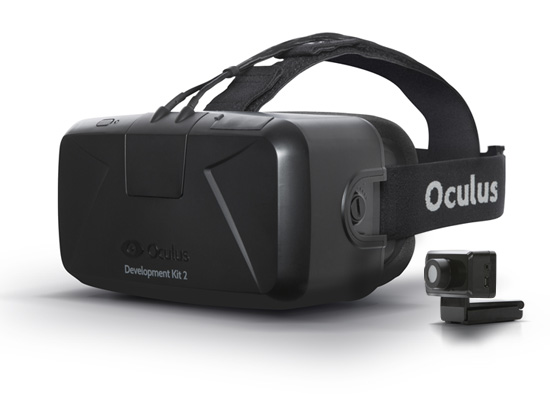
\includegraphics[width=0.5\linewidth]{sections/finalreport/images/dk2.png}	
	\caption{Oculus Rift Development Kit 2 head-mounted display and positional tracker.}
	\label{fig:dk2}
\end{figure}

\subsection{Related  research}
The technique of redirected walking was first introduced by Razzaque et al. in \cite{razzaque}. 
In redirected walking, there are several concepts we can investigate.
There is rotational, translational and curvature redirection.
In addition to these three methods, experiments have been done with dynamic redirection factors.\cite{neth}
In curvature redirection, the virtual world is rotated slightly as the test subject walks forward.
The test subject will then try to correct this rotation which results in him walking on a curved path in the real world while walking on a straight path in the virtual world.
In translational redirection, the virtual distances are altered.
When a test subject moves a distance $d$ in the real world, he walks a distance $d\cdot x$ in the virtual world, for a constant or dynamic factor $x$.
In our experiment, we focus on rotational redirection.
In this type of redirection, the virtual world is rotated when a test subject rotates in the real world.
By exaggerating or reducing the rotation in the virtual world with respect to the rotation in the real world, we can let the user walk tighter or wider turns.

These redirection techniques have been proposed to deal with a limited physical space and a large-scale virtual world.
Consider a room of $x$ by $y$ meters, in which we want to perform an experiment with respect to walking in a virtual world. 
Let the virtual world be a world of size $2x$ by $2y$ meters, now clearly, we can not reach all places in the virtual world when we map the movements in the physical world one-to-one to movements in the virtual world.

Several studies \cite{steinicke2}\cite{steinicke1} have come up with different rotational degrees that could be applied without the user noticing.
In \cite{steinicke2} it is reported that test subjects can be turned about $49\%$ more or $20\%$ less than the perceived virtual rotation. 
In \cite{steinicke1} it is reported that test subjects can be turned about $68\%$ more or $10\%$ less than the perceived virtual rotation. 
\begin{figure}[htb]
	\centering
	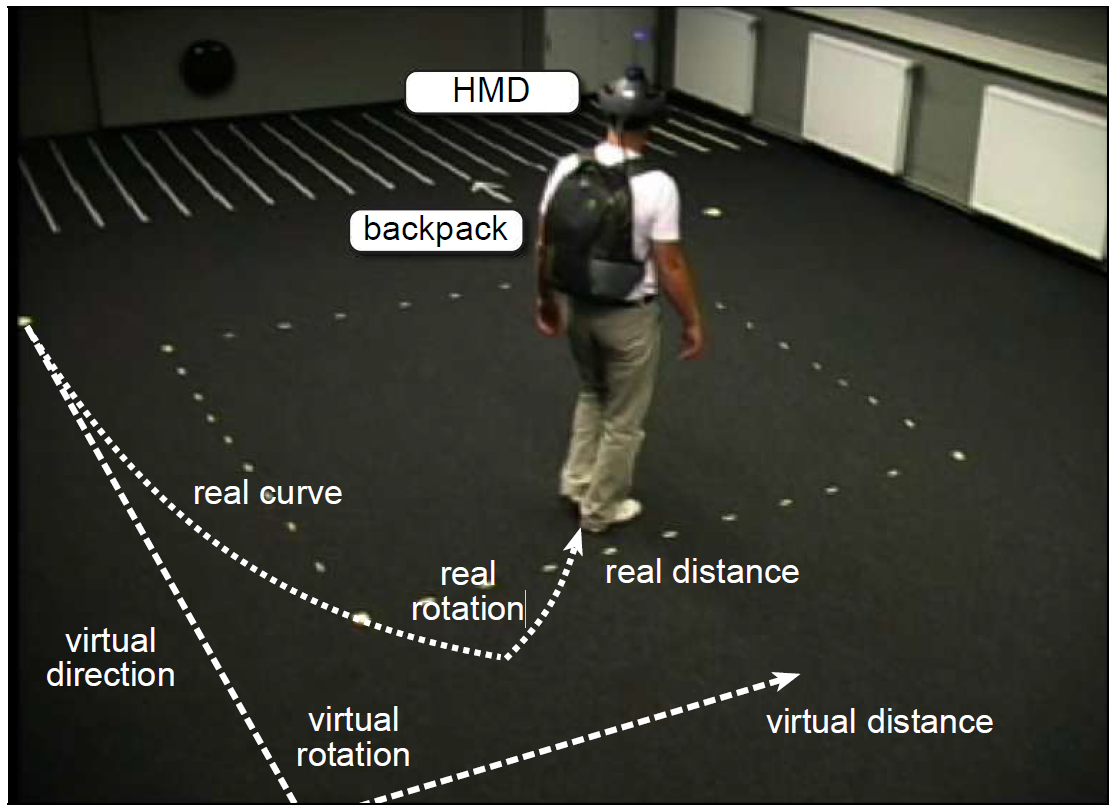
\includegraphics[width=\linewidth]{sections/finalreport/images/steinicke-1.png}	
	\caption{The actual experiment of Steinicke}
\end{figure}
Other studies have investigated the effect of real walking versus other ways of moving forward in the virtual world.
A study by Usoh et al. \cite{usoh} has shown that test subjects that walk in the physical world have a higher presence than so called ``flyers".
In this experiment, the flyers moved forward automatically along their head direction.


